\documentclass[fontsize=12pt]{amsart}
\usepackage[english]{babel}
\usepackage[letterpaper,top=1in,bottom=1in,left=1in,right=1in]{geometry}

\usepackage{amsmath}
\usepackage{graphicx}
\usepackage{xcolor}
\usepackage[colorlinks=true, allcolors=blue]{hyperref}
\usepackage{natbib}


\usepackage{enumitem}
\usepackage{etoolbox}
\usepackage{setspace}
\usepackage{etoolbox}

\title{PROJECT TITLE HERE}
\author{GROUP MEMBERS NAME HERE}
% \date{\today}

\begin{document}
\maketitle


\begin{abstract}
    Write abstract here
\end{abstract}



%%%%%%%%%%%%%%% DELETE THE SECTION BELOW FROM YOUR REPORT 
\section{Learning \LaTeX}


Use the section command like this to make sections in your report. You can also use sub-sections and sub-sub-sections.

For more \LaTeX tips see this tutorial: \href{https://www.overleaf.com/learn/latex/Learn_LaTeX_in_30_minutes}{Learn \LaTeX in 30 Minutes}

\subsection{How to use bibtex for references}

Don't forget to cite things!!! Cite the original paper (if doing type 1 project), cite the textbook if you reference it for ideas, cite other papers if you use them for inspiration, cite links to data if you're using any. 


To cite things, add the bibtex entry to references.bib. 
Then using the bibtex ``key'' (the first thing in the bibtex entry) you can cite it using \cite{haberman_mathematical_1998} which adds the inline citation and adds it to the bibliography.
You can find bibtex entries from google scholar -- \href{https://libguides.usask.ca/c.php?g=218034&p=1445751}{this link shows you how}. 

You can refer to figures using their labels. For example, Figure \ref{fig:Bella} shows a picture of my dog, Bella.

Feel free to change any of the section names if appropriate and add subsections. 


\textcolor{red}{All of the above should be deleted when you write your report. Your report should start with the introduction}
%%%%%%%%%%%%%%% DELETE THE ABOVE SECTION FROM YOUR REPORT 




%% 
\section{Introduction}

This is the introduction. 
\section{Background}

Write background here

\section{Our Model}

Describe your model

\section{Results}

Reults?

\begin{figure}
    \centering
    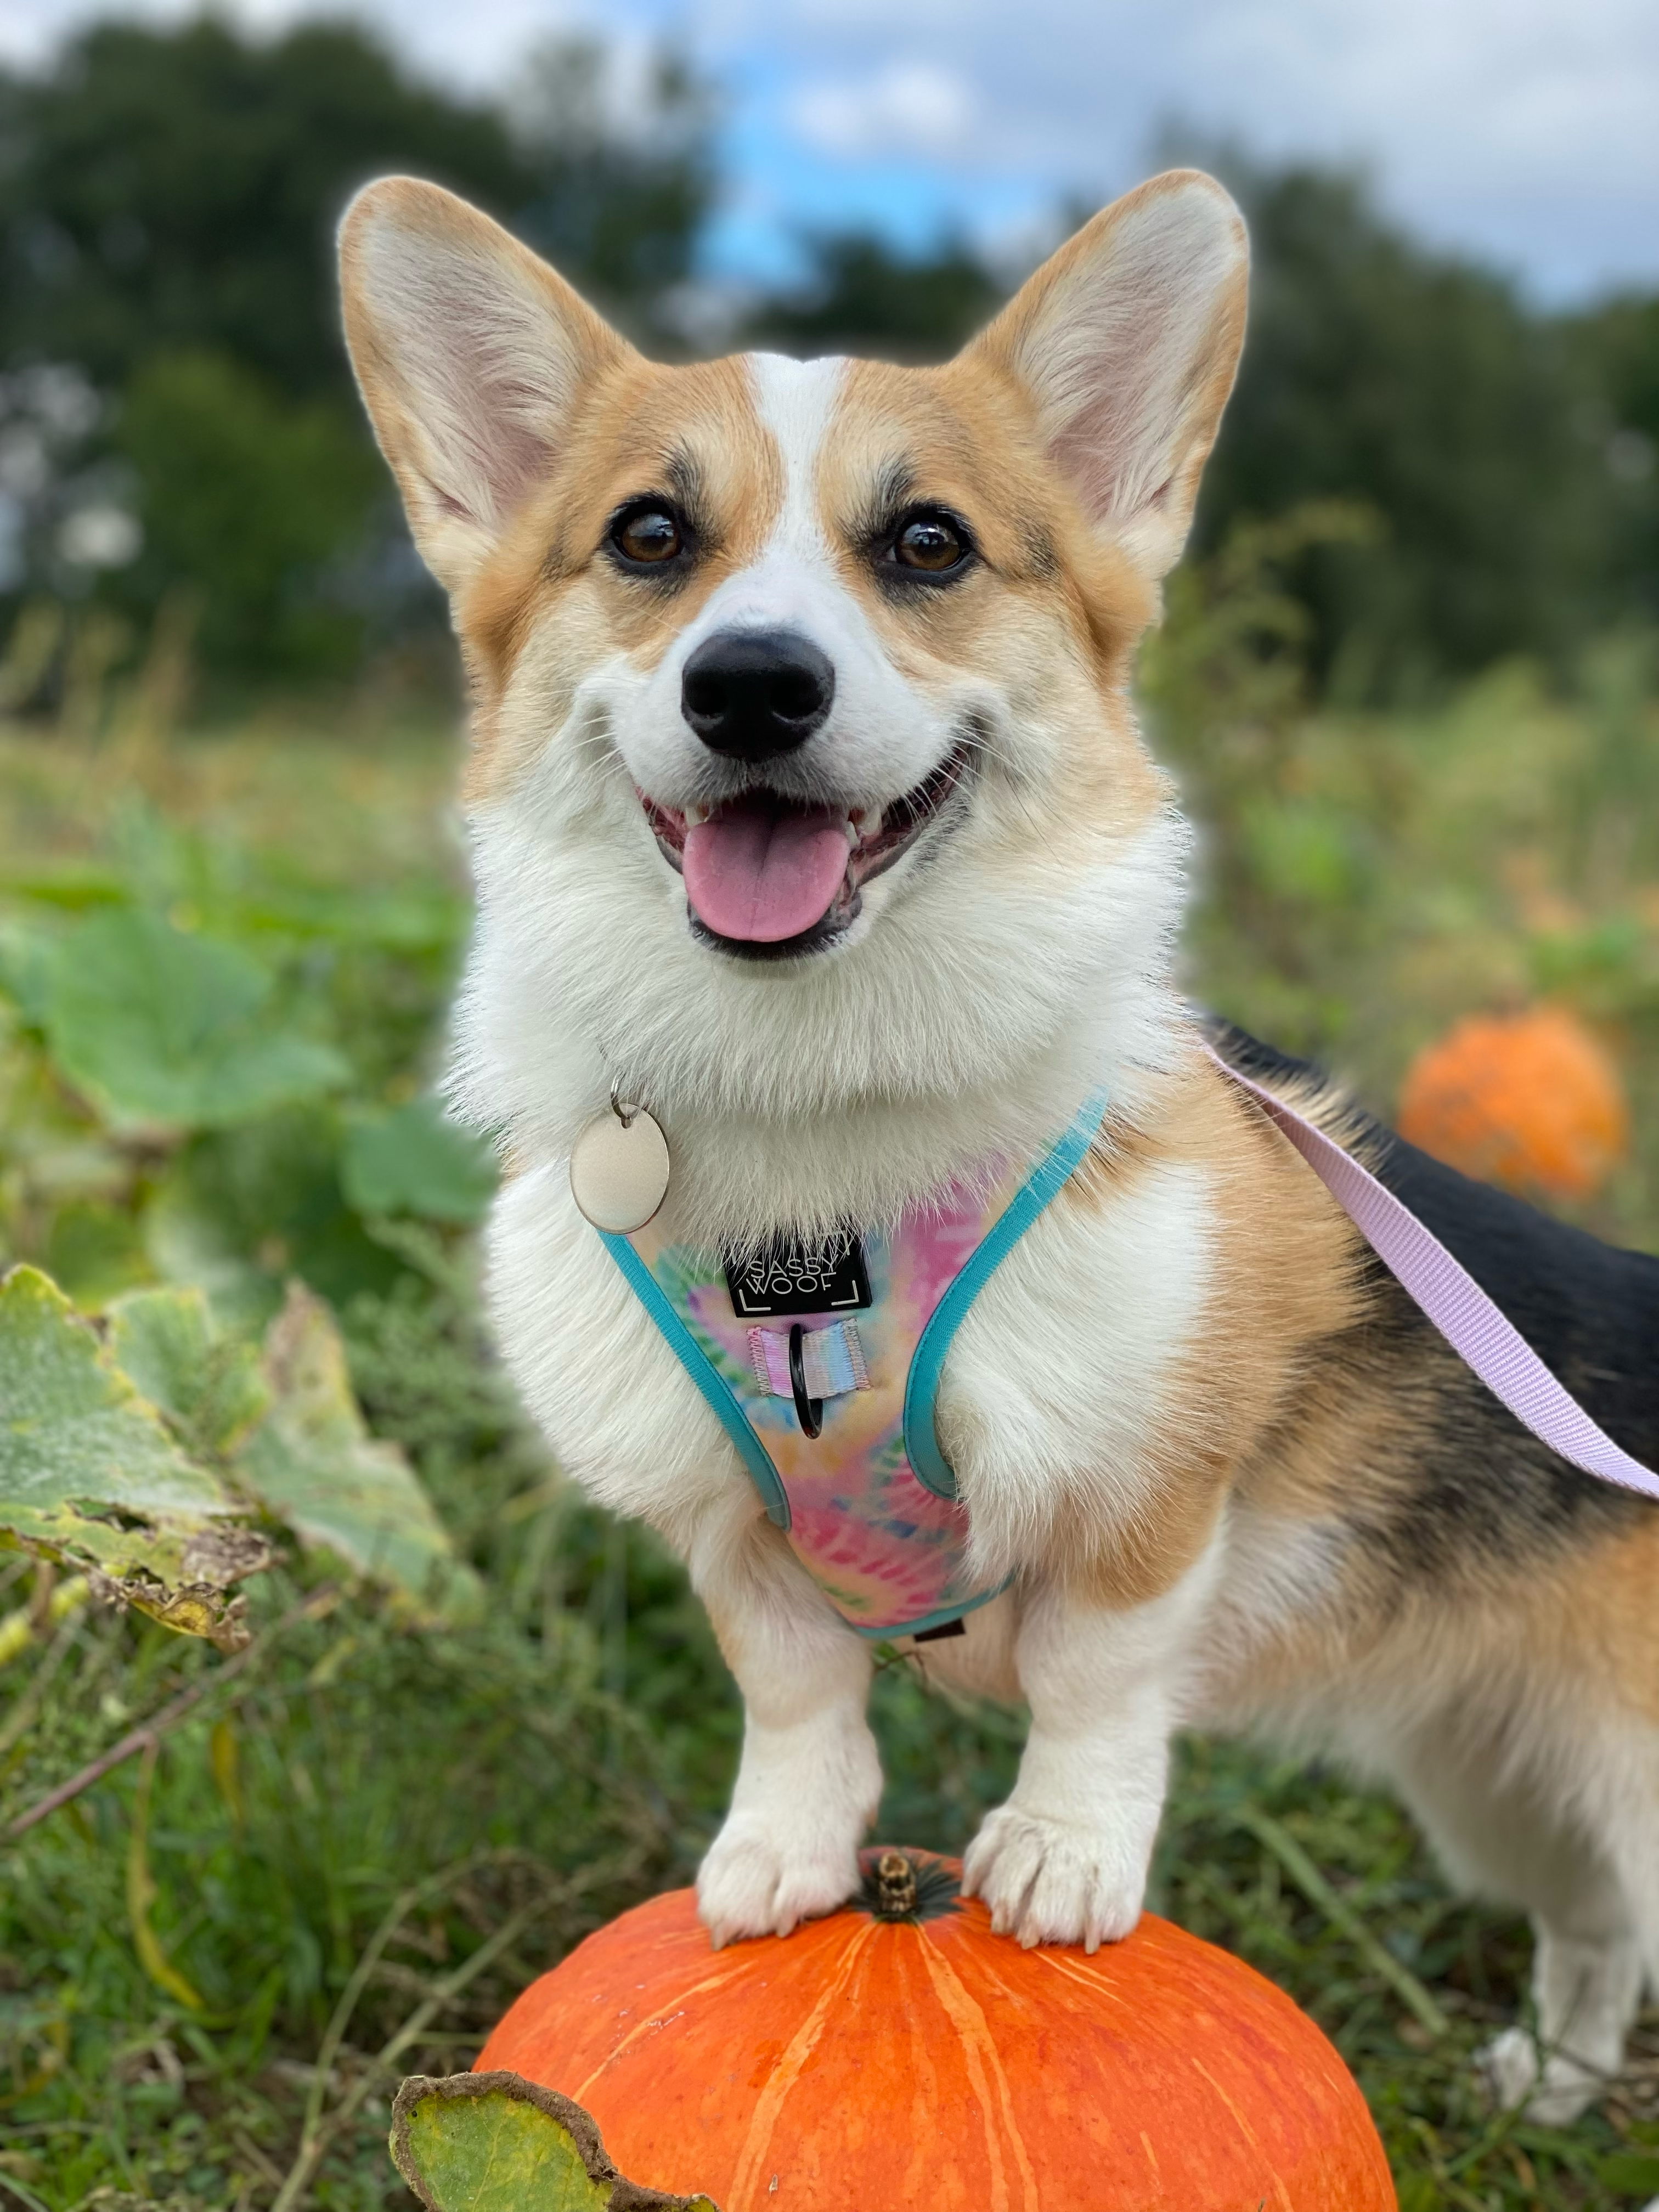
\includegraphics[width=0.4\textwidth]{Bella.png} % put name of image file in the {}
    \caption{Here's how to make a figure with a caption!}
    \label{fig:Bella}
\end{figure}

\section{Conclusions and Discussion}
The conclusion goes here.


\bibliographystyle{abbrv}
\bibliography{references}


\section*{Acknowledgements}

Did you get any help on this project? Did a classmate give you advice? Or a friend help edit your writing? Did the TA help? Acknowledge any of these people here.

 
\appendix
\section{Group Contributions}

% This appendix section is REQUIRED

\textbf{Name of Group Member}: Describe contributions here.

\textbf{Name of Group Member}: Describe contributions here.

\textbf{Name of Group Member}: Describe contributions here.

\textbf{Name of Group Member}: Describe contributions here.


\section{title of optional appendix (if needed)}
appendix goes here (if needed)



\end{document}